% --------------------------------------------------------------
% This is all preamble stuff that you don't have to worry about.
% Head down to where it says "Start here"
% --------------------------------------------------------------
 
\documentclass[12pt]{article}
 
\usepackage[margin=1in]{geometry} 
\usepackage{amsmath,amsthm,amssymb, stix}
\usepackage{hyperref}
\usepackage{booktabs}
\usepackage[table]{xcolor}
\usepackage{graphicx}
\usepackage{subcaption}
\usepackage[htt]{hyphenat}
\usepackage{listings}
\usepackage{minted}
\usepackage{booktabs} % For better looking tables
\usepackage{array}    % For better column formatting
 
\newcommand{\N}{\mathbb{N}}
\newcommand{\Z}{\mathbb{Z}}
 
\newenvironment{theorem}[2][Theorem]{\begin{trivlist}
\item[\hskip \labelsep {\bfseries #1}\hskip \labelsep {\bfseries #2.}]}{\end{trivlist}}
\newenvironment{lemma}[2][Lemma]{\begin{trivlist}
\item[\hskip \labelsep {\bfseries #1}\hskip \labelsep {\bfseries #2.}]}{\end{trivlist}}
\newenvironment{exercise}[2][Exercise]{\begin{trivlist}
\item[\hskip \labelsep {\bfseries #1}\hskip \labelsep {\bfseries #2.}]}{\end{trivlist}}
\newenvironment{problem}[2][Problem]{\begin{trivlist}
\item[\hskip \labelsep {\bfseries #1}\hskip \labelsep {\bfseries #2.}]}{\end{trivlist}}
\newenvironment{question}[2][Question]{\begin{trivlist}
\item[\hskip \labelsep {\bfseries #1}\hskip \labelsep {\bfseries #2.}]}{\end{trivlist}}
\newenvironment{corollary}[2][Corollary]{\begin{trivlist}
\item[\hskip \labelsep {\bfseries #1}\hskip \labelsep {\bfseries #2.}]}{\end{trivlist}}

\newenvironment{solution}{\begin{proof}[Solution]}{\end{proof}}
 
\begin{document}
 
% --------------------------------------------------------------
%                         Start here
% --------------------------------------------------------------
 
\title{Assignment 2: Machine Translation}
\author{Singh Karanbir\\ %replace with your name
Advanced Natural Language Processing and Deep Learning}

\maketitle

\section{Assignment description}
In this exercise, I replicated some of the experiments in one of the submissions to the shared task on Unsupervised MT and Very Low Resource Supervised MT at WMT 2022.

Specifically, the task is to replicate the experiments on translation between Upper Sorbian and Lower Sorbian described in the following paper:

\vspace{0.5cm}
\textit{Edoardo Signoroni and Pavel Rychlý (2022). MUNI-NLP Systems for Lower Sorbian-German and Lower Sorbian-Upper Sorbian Machine Translation @WMT22. In: Proceedings of the Seventh Conference on Machine Translation (WMT), Abu Dhabi, pp. 1111–1116.}
\href{https://aclanthology.org/2022.wmt-1.109/}{https://aclanthology.org/2022.wmt-1.109/}
\vspace{0.5cm}

The datasets are found here:

\href{https://www.statmt.org/wmt22/unsup_and_very_low_res.html}{https://www.statmt.org/wmt22/unsup\_and\_very\_low\_res.html}

\section{Data}
The \textbf{hsb} (Upper Sorbian) and \textbf{dsb} (Lower Sorbian) parts of the corpus are in two separate files. 

The "\textit{train\_dsb\_hsb\_62564}" files are the training data; 
the "\textit{valid\_dsb\_hsb}" files are the validation set; and the "\textit{dev\_dsb\_hsb\_new}" files are the test set.

The two languages are quite similar (\textit{see Figure 1 and Figure 2}): this aspect is discussed in the last part of this report (the system improvement with \textbf{hft}).

\begin{figure}
    \begin{minipage}{.5\textwidth}
      \centering
      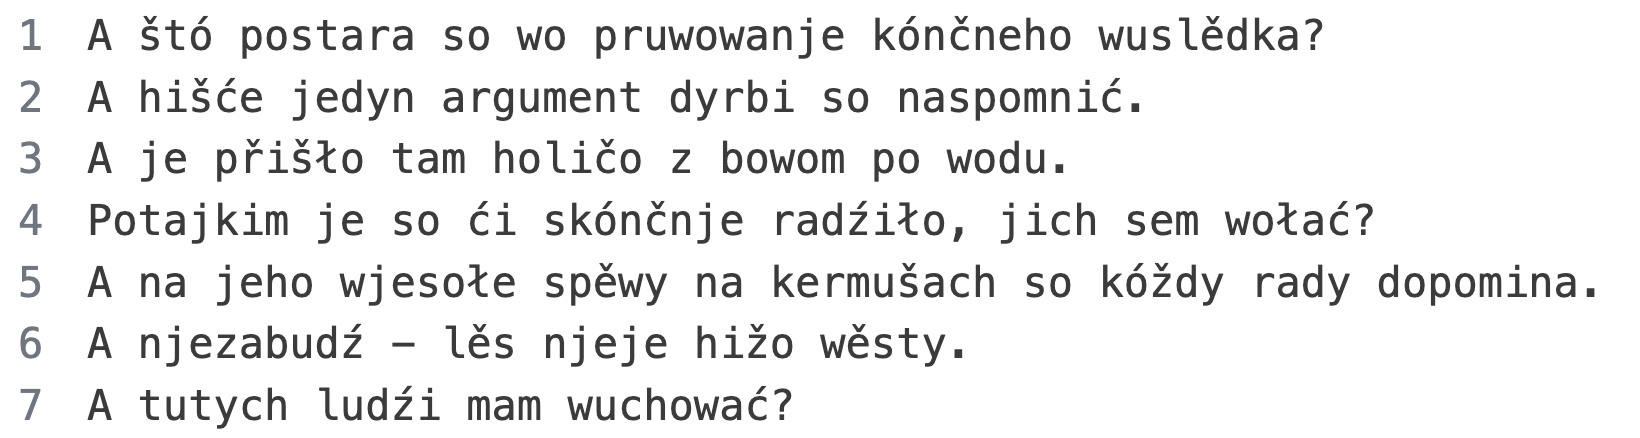
\includegraphics[width=1\linewidth]{report/figures/hsb-example.png}
      \captionof{figure}{Upper Sorbian}
      \label{fig:hsb-example}
    \end{minipage}%
    \begin{minipage}{.5\textwidth}
      \centering
      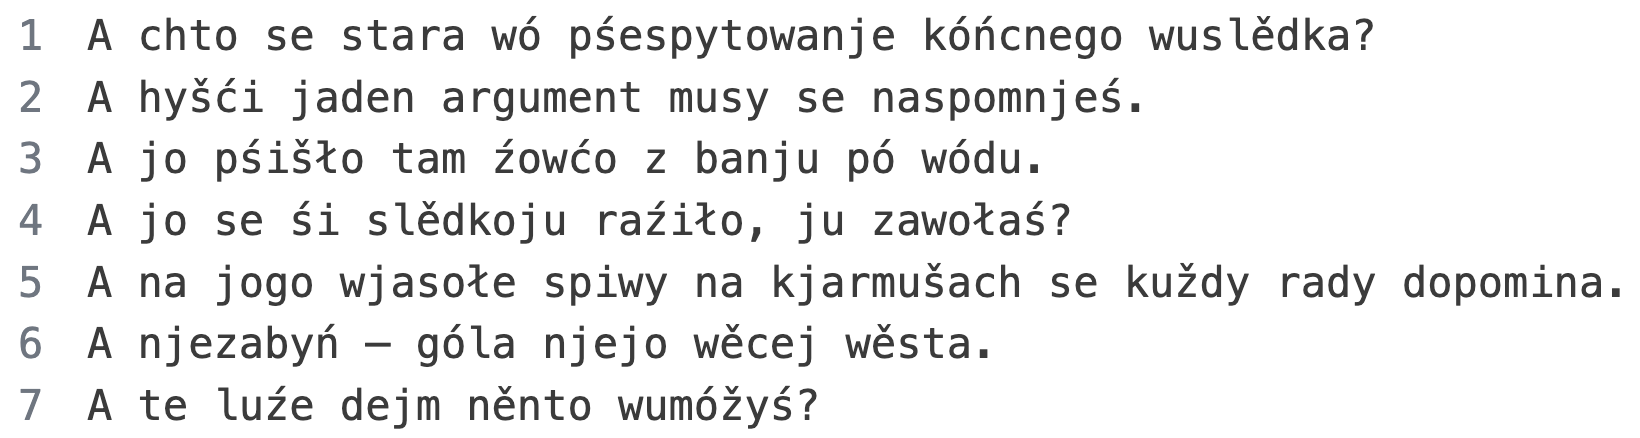
\includegraphics[width=1\linewidth]{report/figures/dsb-example.png}
      \captionof{figure}{Lower Sorbian}
      \label{fig:dsb-example}
    \end{minipage}
\end{figure}

\section{Data preparation and Baseline training}
\subsection{Train BPE vocabularies}
\textbf{BPE} (Byte Pair Encoding) training is the process of building a subword vocabulary for a text tokenizer by repeatedly finding and merging the most frequent pairs of adjacent characters or tokens in a given text corpus.

For training BPE, it was asked to use \texttt{subword-nmt}\footnote{\href{https://github.com/rsennrich/subword-nmt}
{https://github.com/rsennrich/subword-nmt}} and I've done it in this way:

\vspace{0.5cm}
\texttt{
  subword-nmt learn-joint-bpe-and-vocab --input train\_dsb\_hsb\_62564.dsb train\_dsb\_hsb\_62564.hsb -s 4000 -o trained\_bpe --write-vocabulary vocab.dsb vocab.hsb
}

The command above gives us the trained BPE of size more or less 4000 and two separate vocabularies from the given train data.

After this, I've applied the learned BPE to all datasets, with this command (\textit{it's only an example for only one file}):

\vspace{0.5cm}
\texttt{
  subword-nmt apply-bpe -c trained\_bpe --vocabulary vocab.dsb --vocabulary-threshold 50 < dev\_dsb\_hsb\_new.dsb > dev\_dsb\_hsb\_new.BPE.dsb
}

\subsection{Data preprocessing for Fairseq}
We must generate the binary files needed for \textbf{Fairseq}\footnote{\href{https://fairseq.readthedocs.io/en/latest/index.html}{https://fairseq.readthedocs.io/en/latest/index.html}, \href{https://github.com/facebookresearch/fairseq}{https://github.com/facebookresearch/fairseq}}, the sequence modeling toolkit we are going to use for our machine translation task.

\vspace{0.5cm}
\texttt{
    fairseq-preprocess --source-lang dsb --target-lang hsb --trainpref train\_dsb\_hsb\_62564.BPE --validpref valid\_dsb\_hsb.BPE --testpref dev\_dsb\_hsb\_new.BPE --destdir dsb-to-hsb --srcdict vocab.dsb --tgtdict vocab.hsb
}

\vspace{0.2cm}
{\centering
(\textit{Note that this is done for \textbf{dsb} $\rightarrow$ \textbf{hsb}, the same has to be done for \textbf{hsb} $\rightarrow$ \textbf{dsb}})\par
}

\subsection{Train Fairseq}
Now, we can train the model running this command:

\vspace{0.2cm}
\texttt{
fairseq-train dsb-to-hsb --arch transformer --encoder-layers 5 --decoder-layers 5 --encoder-ffn-embed-dim 1024 --decoder-ffn-embed-dim 1024 --encoder-attention-heads 2 --decoder-attention-heads 2 --dropout 0.3 --attention-dropout 0.3 --activation-dropout 0.3 --encoder-layerdrop 0.1 --decoder-layerdrop 0.1 --optimizer adam --clip-norm 1.0 --lr 0.0005 --lr-scheduler inverse\_sqrt --criterion label\_smoothed\_cross\_entropy --label-smoothing 0.5 --max-tokens 4096 --save-dir ./dsb-to-hsb/t-opt-bpe/checkpoints --patience 10}

\newpage

The hyperparameters are set following the paper (reported in Figure 3):
in this particular case, \textit{t-bpe} training as described
may require too much GPU memory, so I've considered to train the smaller \textit{t-opt-bpe} to make the model fit on the GPUs we have, at cost in system performance.

\begin{figure}
    \centering
    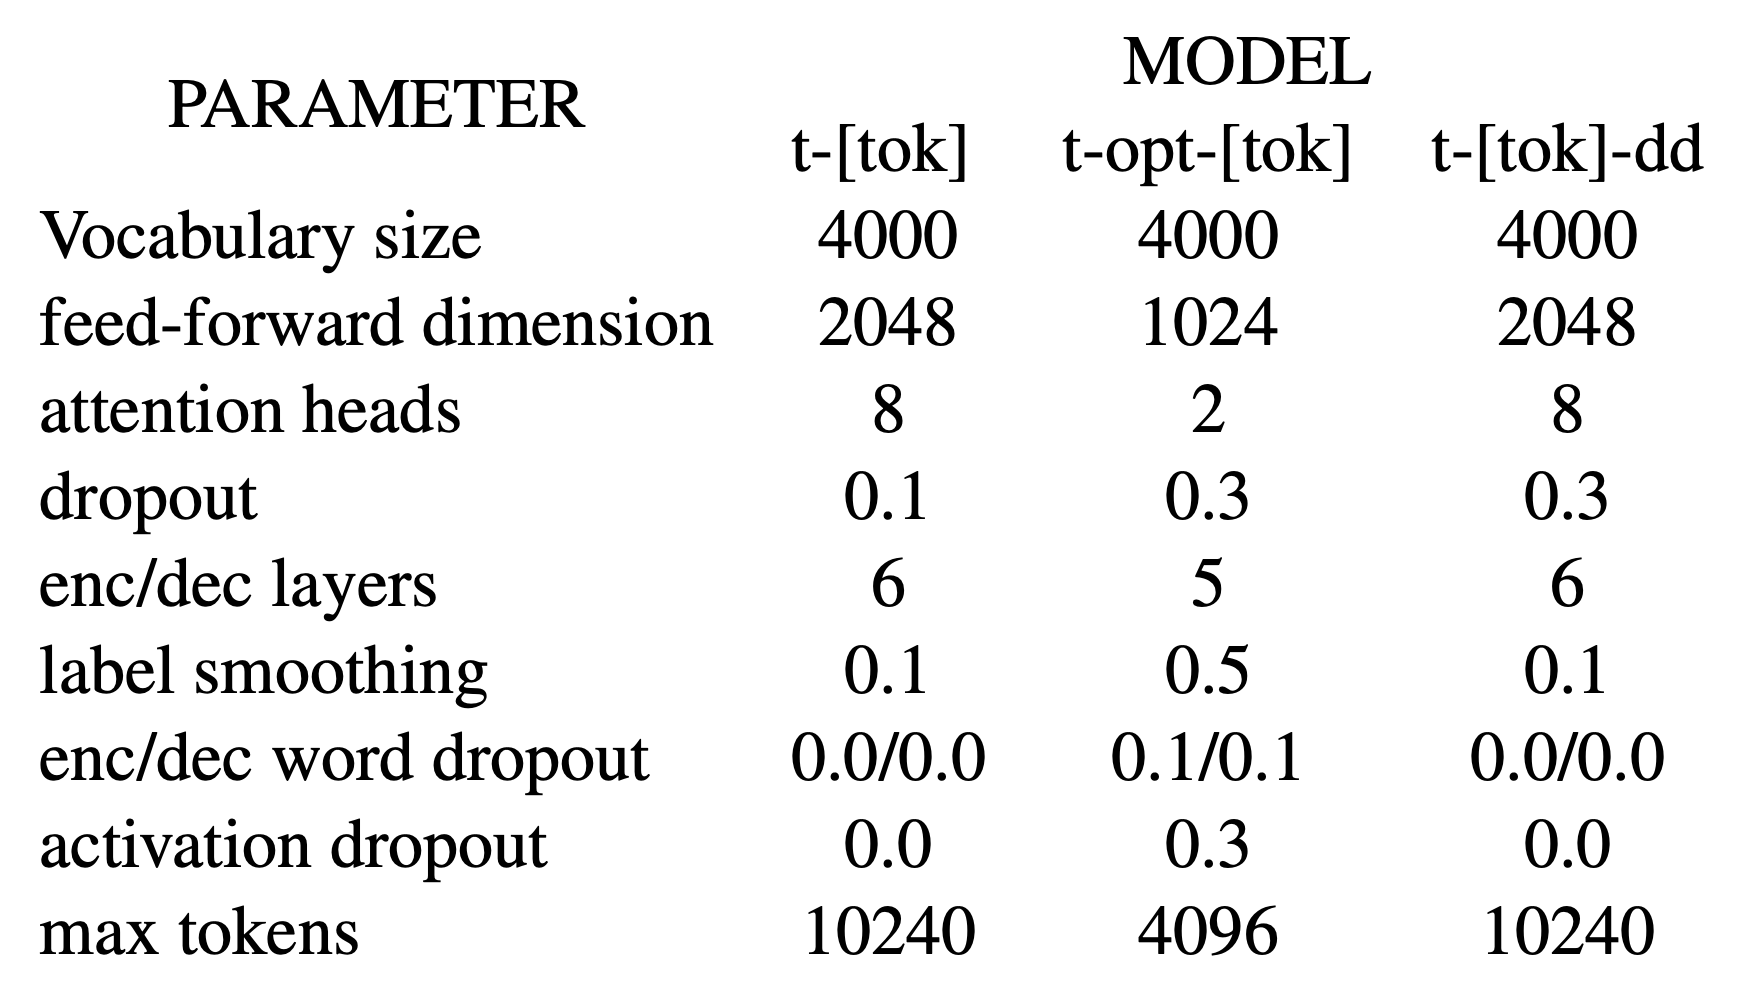
\includegraphics[width=0.7\linewidth]{report/figures/hyperparameters.png}
    \caption{Model hyperparameters}
    \label{fig:hyperparameters}
\end{figure}

\subsection{Generate translations}
After the model is trained, we generate translations of test data from which we extract the MT system output and the reference translation. Here is the command:

\vspace{0.2cm}
\texttt{
fairseq-generate dsb-to-hsb --path checkpoint\_best.pt --batch-size 128 --beam 5}

\vspace{0.2cm}
\texttt{grep '\^H' fairseq.out | cut -f3- > system.out \#Extract model translations}

\texttt{grep '\^T' fairseq.out | cut -f2- > reference.out \#Extract translations reference}

\vspace{0.2cm}
We must detokenize for getting clean translations and also for computing the BLEU score:

\vspace{0.2cm}
\texttt{sed -r 's/(@@ )|(@@ ?\$)//g' system.out > system.out.detok}

\texttt{sed -r 's/(@@ )|(@@ ?\$)//g' reference.out > reference.out.detok}

\vspace{0.2cm}
{\centering
(\textit{As before, note that this is done for \textbf{dsb} $\rightarrow$ \textbf{hsb}, the same has to be done for \textbf{hsb} $\rightarrow$ \textbf{dsb}})\par
}

\subsection{Compute BLEU score}
Finally, we can compute BLEU, an algorithm for evaluating the quality of text which has been machine-translated from one natural language to another, using this command:

\vspace{0.2cm}
\texttt{
sacrebleu reference.out.detok < system.out.detok
}

\section{System Development}
Signoroni and Rychlý describe two methods, with which they achieved (minor) improvements in system performance: \textbf{High Frequency Tokenisation (HFT)} and \textbf{Data Diversification (DD)}.

I've decided to implement HFT: details and implementation below.

\subsection{High Frequency Tokenisation}
High Frequency Tokenisation (HFT) is a subword splitting method that the authors claim works better in low-resource scenario. 

The steps are already described in the paper, but I've decided to implement a slightly different version of HFT:
instead of using the \textbf{$<$explicit-whitespace$>$}, I'm just putting the \textbf{$<$token-delimiter$>$} between tokens. 
An example is reported in Figure 4.

\begin{figure}
    \centering
    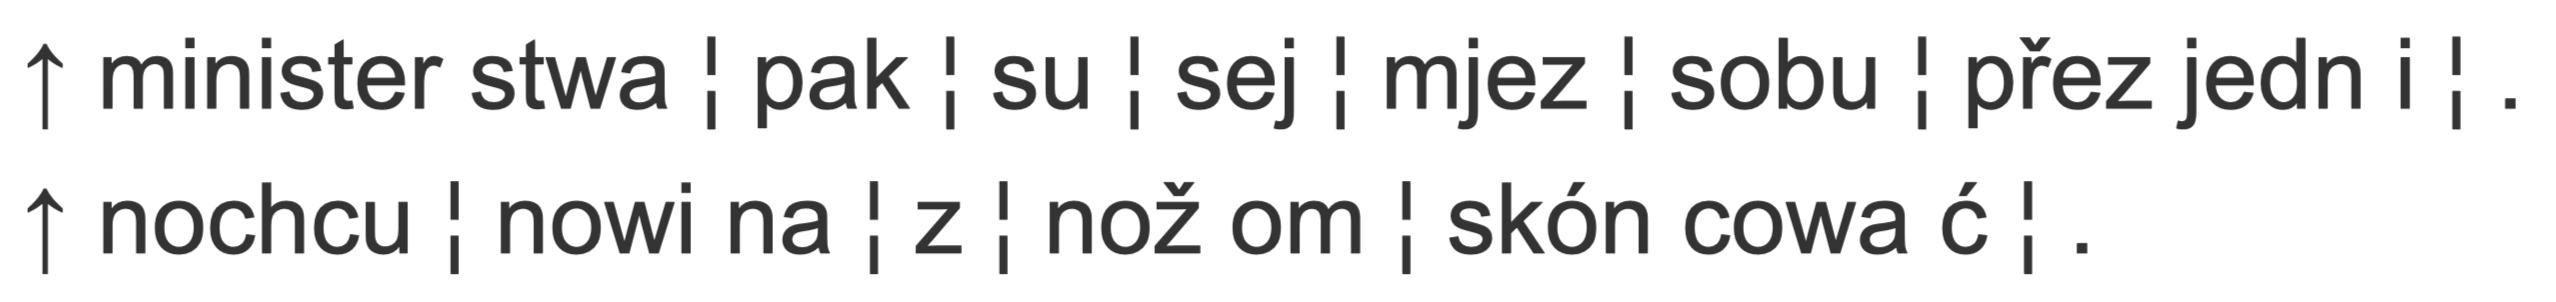
\includegraphics[width=0.7\linewidth]{report/figures/hft_example.png}
    \caption{My version of HFT encoding}
    \label{fig:hft_example}
\end{figure}


At the end of the day, it's quite similar to the original HFT implementation and gives also similar results of the paper. 

Moreover, since the two languages are alike I've decided to build a single vocabulary from a joint train data.

\subsubsection{Implementation}
Here the main functions for HFT Tokenisation.

\begin{minted}
[
frame=lines,
framesep=1mm,
baselinestretch=0.9,
fontsize=\footnotesize,
linenos
]
{python}
def learn_hft(input_file: str, target_vocab_size=4000, k_fraction=0.05) -> Dict:
    """
    Learn HFT vocabulary from an input file.

    Args:
        input_file (str): the file from which the vocabulary is learned 
        target_vocab_size (int, optional): wanted vocabulary size. 
        Defaults to 4000.
        k_fraction (float, optional): fraction of the target vocabulary size. 
        Defaults to 0.05.

    Returns:
        Dict: learned vocabulary
    """
    # Initial vocabulary = all characters
    char_counts = Counter()
    for tokens in load_stream(input_file):
        for token in tokens:
            for ch in token:
                char_counts[ch] += 1
    vocab = dict(char_counts) # {token: freq}

    # Represent each token as a list of current subwords
    segmented_tokens = []
    for tokens in load_stream(input_file):
        segmented_line = []
        for token in tokens:
            segmented_line.append(list(token))
        segmented_tokens.append(segmented_line)

    # Loop until reaching target vocab size
    while len(vocab) < target_vocab_size:
        # Count subword frequencies and candidate pairs
        subword_freq = Counter()
        pair_freq = Counter()
        for line in segmented_tokens:
            for token_subwords in line:
                # Subword frequencies
                for subword in token_subwords:
                    subword_freq[subword] += 1
                    
                # Pairs
                for i in range(len(token_subwords) - 1):
                    pair = (token_subwords[i], token_subwords[i+1])
                    pair_freq[pair] += 1

        # Select top K candidates
        k = max(1, int(k_fraction * (target_vocab_size - len(vocab))))
        top_pairs = pair_freq.most_common(k)
        if not top_pairs:
            # print("No more pairs to merge.")
            break

        # Merge subwords according to top pairs
        merges = {pair: pair[0] + pair[1] for pair, _ in top_pairs}
        
        # Add to vocab
        for pair, freq in top_pairs:
            new_token = merges[pair]
            vocab[new_token] = freq

        # Remove rare subwords
        min_freq = top_pairs[-1][1]
        for token in list(vocab.keys()):
            if len(token) > 1 and vocab[token] < min_freq:
                del vocab[token]

        # Update segmented tokens
        for line in segmented_tokens:
            for i, token_subwords in enumerate(line):
                j = 0
                new_subwords = []
                while j < len(token_subwords):
                    if j < len(token_subwords)-1:
                        pair = (token_subwords[j], token_subwords[j+1])
                        if pair in merges:
                            new_subwords.append(merges[pair])
                            j += 2
                            continue
                    new_subwords.append(token_subwords[j])
                    j += 1
                line[i] = new_subwords
    return vocab
\end{minted}

Explanation:
\begin{itemize}
    \item \textbf{\texttt{load\_stream()}}: \textbf{pretokenize} the input file, line by line; sentences are split into tokens on the borders of alphanumeric and non-alphanumeric characters and then applies case normalization
    
    \item \textit{Line 16-21}: initialize the vocabulary with single characters and their frequencies from pretokenized input file

    \item \textit{Line 24-29}: saves in \texttt{segmented\_tokens} a list of lists of tokens characters from pretokenized input file, this will be useful for when we start merging subwords 
    
    {\centering
    \texttt{"This is good"} $\rightarrow$ \texttt{[[[T,h,i,s], [i,s], [g,o,o,d]]]}
    \par}

    \item \textit{Line 34-35}: for each line, we save the frequency of each subword and of the pair formed by the concatenation of the current subword and next one

    \item \textit{Line 48-52}: select the top K candidates from the pair frequencies dictionary

    \item \textit{Line 55-60}: from the top K candidates, merge subwords and add it into the vocabulary

    \item \textit{Line 63-66}: update vocabulary, removing rare subwords considered as such if they have frequency less then the minimum frequency among the top K candidates

    \item \textit{Line 69-82}: we need to update \texttt{segmented\_tokens} with the merges we found so far

    {\centering
    \texttt{[g,o,o,d]} $\rightarrow$ \texttt{[go,o,d]} $\rightarrow$ \texttt{[goo,d]} and so on
    \par}

    \item \textit{Repeat from line 33 until we reach the vocabulary target size}
\end{itemize}

\begin{minted}
[
frame=lines,
framesep=1mm,
baselinestretch=0.9,
fontsize=\footnotesize,
linenos
]
{python}
def encode(self, text: str) -> List[str]:
        """
        Encode text into a list of subword tokens with proper case and delimiters handling.

        Args:
            text (str): text that needs to be encoded

        Returns:
            List[str]: list of subwords and delimiters (the encoded text). Example: "↑ tam ¦ pśe póda jo ¦ koncer n ¦ tak ¦ pomjen jony ¦ awto ¦ ."
        """
        # Split into words and non-words and mantain whitespaces
        tokens = re.findall(r'\w+|[^\w\s]|\s+', text)
        tokens = [t for t in tokens if t.strip() or t == ' ']
        
        subwords = []
        for i, token in enumerate(tokens):
            if token.isspace():
                # Add delimiter for whitespace (except at beginning)
                if i > 0 and subwords and subwords[-1] != TOKEN_DELIM:
                    subwords.append(TOKEN_DELIM)
                continue
            
            # Add delimiter before each token (except the first)
            if i > 0 and not tokens[i-1].isspace() and subwords and subwords[-1] != TOKEN_DELIM:
                subwords.append(TOKEN_DELIM)
            
            if token.isalpha():
                # Alphabetic token
                if token.isupper() and len(token) > 1:
                    # All uppercase word
                    segments = self.segment_token(token)
                    subwords.append(ALL_UPPER)
                    subwords.extend(segments)
                    subwords.append(END_UPPER)
                elif token.istitle() or (len(token) == 1 and token.isupper()):
                    # Title case or single uppercase
                    segments = self.segment_token(token)
                    subwords.append(SINGLE_UPPER)
                    subwords.extend(segments)
                else:
                    # Lowercase or mixed case (treat as lowercase for segmentation)
                    segments = self.segment_token(token)
                    subwords.extend(segments)
            else:
                # Punctuation or numbers - segment as is
                segments = self.segment_token(token)
                subwords.extend(segments)
                
        return subwords
\end{minted}

\begin{itemize}
    \item \texttt{segment\_token()}: segments token based on the vocabulary and merges we've learned before

    {\centering
    \texttt{"namakajomy" $\rightarrow$ ["nama", "ka", "jomy"]}
    \par}

    \item \textit{Line 15-47}: handle delimiters
    
    {\centering
    \texttt{"Hello WORLD!" $\rightarrow$ [$\uparrow$,h,ell,o,¦,$\triangledown$,wor,l,d,$\vartriangle$,¦,!]}
    \par}

\end{itemize}

\begin{minted}
[
frame=lines,
framesep=1mm,
baselinestretch=0.9,
fontsize=\footnotesize,
linenos
]
{python}
def decode(self, encoded_text: str) -> str:
        """
        Decode tokens back into text by reversing markers.

        Args:
            encoded_text (str): text to decode. Example: "↑tam¦pśepódajo¦koncern¦tak¦pomjenjony¦awto¦."

        Returns:
            str: decoded text, without delimiters and other special characters used for tokenization
        """
        result = []
        
        i = 0
        while i < len(encoded_text): # ↑tam jo koncern pśepódał tak pomjenjony awto .
            token = encoded_text[i]
            i += 1
            
            # The token delimeter is equal to have a whitespace (even if it's not totally correct, but it works well)
            if token == TOKEN_DELIM:
                result.append(' ')
                
            elif token == ALL_UPPER:
                uppercase_buffer = []


                
                # Save token's characaters in the uppercase buffer
                while i < len(encoded_text) and encoded_text[i] != END_UPPER:
                    uppercase_buffer.append(encoded_text[i])
                    i += 1
                    
                # Convert to uppercase and add to result
                if uppercase_buffer:
                    uppercase_word = ''.join(uppercase_buffer).upper()
                    result.append(uppercase_word)
                    
                # Skip the END_UPPER marker
                if i < len(encoded_text) and encoded_text[i] == END_UPPER:
                    i += 1
                    
            elif token == SINGLE_UPPER:
                if i < len(encoded_text):
                    # Capitalize the next token
                    next_token = encoded_text[i]
                    if len(next_token) == 1:
                        result.append(next_token.upper())
                    else:
                        # For multicharacter tokens, capitalize first letter
                        result.append(next_token[0].upper() + next_token[1:])
                    i += 1
            else:
                # Regular token
                result.append(token)
                
        # Join and clean up spaces around punctuation
        text = ''.join(result)
        
        # Fix spacing around punctuation
        text = re.sub(r'\s+([.,!?;:])', r'\1', text)  # Remove space before punctuation
        text = re.sub(r'([.,!?;:])\s+', r'\1 ', text)  # Ensure space after punctuation
        return text.strip()
\end{minted}

I'm not going to describe line per line what the \texttt{decode()} function does: simply it takes the encoded text, removes delimiters and builds the original text.

{\centering
    \texttt{"$\uparrow$h ell o¦$\triangledown$wor l d$\vartriangle$¦ !" $\rightarrow$ "Hello WORLD!"}
    \par}

\newpage

\section{Evaluation}
\begin{table}[htbp]
\centering

\begin{tabular}{lccccc}
\toprule
 & \textbf{DSB $\rightarrow$ HSB} & \textbf{HSB $\rightarrow$ DSB} \\
\midrule
\textbf{t-opt-bpe} & 71.37 & 69.50 \\
\textbf{t-opt-bpe} (\textit{mine}) & 68.9 & 67.7 \\
\midrule
\textbf{t-opt-hft} & 71.83 & 68.95 \\
\textbf{t-opt-hft} (\textit{mine}) & 70.8 & 68.3 \\
\bottomrule
\end{tabular}
\caption{Results}
\label{tab:results}
\end{table}

\end{document}